\documentclass[12pt,letterpaper]{report}
\usepackage[utf8]{inputenc}
\usepackage{amsmath} % For equations
\usepackage{amsfonts} % Math fonts
\usepackage{amssymb} % Math symbols
\usepackage{capt-of} % To use \captionof
\usepackage{graphicx} % For pictures
\usepackage{caption} % To bold all captions
\usepackage{pgfplotstable} % Generates table from .csv
\usepackage{pgfplots} % Generate plots
\usepackage{titlesec} % To reformat chapter headings
\usepackage[obeyspaces]{url} % Url formatting
\usepackage{geometry} % To make margins smaller
\usepackage{booktabs}
\usepackage{float}
\usepackage{placeins}

\usepackage{listings}
\usepackage{color}
\definecolor{pblue}{rgb}{0.13,0.13,1}
\definecolor{pgreen}{rgb}{0,0.5,0}
\definecolor{pred}{rgb}{0.9,0,0}
\definecolor{pgrey}{rgb}{0.46,0.45,0.48}
\lstset{ %
	showtabs=false,
	breaklines=true,
	showstringspaces=false,
	commentstyle=\color{pgreen},
	keywordstyle=\color{pblue},
	stringstyle=\color{pred},
	basicstyle=\ttfamily,
	moredelim=[il][\textcolor{pgrey}]{\$\$},
	moredelim=[is][\textcolor{pgrey}]{\%\%}{\%\%},
	frame=single,
	title=\lstname,
}
\author{Jose Perez}
\title{[CS 4365/5354] Deep Learning - Lab 1 Report}
\date{September 7th, 2017}

% Remove the word Chapter
\titleformat{\chapter}% reformat chapter headings
	[hang]% like section, with number on same line
	{\Huge\bfseries}% formatting applied to whole
	{\thechapter.}% Chapter number
	{0.5em}% space between # and title
	{}% formatting applied just to title

% Inserts two lines to sign name and date
\newcommand*{\signature}[1]{%
	\par\noindent\makebox[2.5in]{\hrulefill} \hfill\makebox[2.0in]{\hrulefill}%
	\par\noindent\makebox[2.5in][l]{#1}      \hfill\makebox[2.0in][l]{Date}%
}%

\begin{document}
	% Bold captions
	\captionsetup{labelfont=bf}
	% Title Page
	\pagenumbering{gobble} % Disable page numbering
	\maketitle
	\pagenumbering{arabic} % Re-enable page numbering
	\newpage
    
	\tableofcontents
	\chapter{Lab 1}

	\paragraph{Problem}
		Implement the feed-forward part of a neural network with a given architecture, weights, and biases to classify the MNIST dataset.

	\section{Solution Design and Implementation}	
    	I implemented the neural network in Python with the help of the numpy library, following the guidelines of the specified architecture of each layer and translating the operations to their numpy equivalent.
        
   		The non-linear functions used were ReLU and Sigmoid. I implemented my own ReLU function and used the scipy expit function for the sigmoid.
        
        To generate the confusion matrix from my experiment I used scipy.
        
        I created a small interactive matplotlib figure that went through the misclassified digits using the arrow keys to go through and get interesting misclassified digits.

	% Experimental Results - Describe experiments performed to test program and show output produced
	% Must be described in a way that allows anybody to replicate them
	% Include sample runs that illustrate outputs and running time under different types of inputs
	\section{Experiments}
The computer used to run these experiments is a Dell Inspiron 13 which has an Intel i7 Core and 12GB of memory.
    
The accuracy of the classification was 97.94\%.
    
The program takes on average 12 seconds to run. On average 8 of those are loading the files.
    
    \subsection{Confusion Matrix}
    	
    \begin{figure}[H]
   	\centering
    \scalebox{0.8}{
    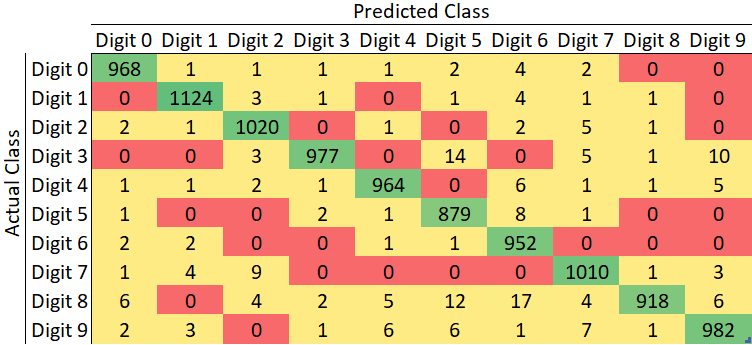
\includegraphics[width=\linewidth]{lab1_conf_matrix.png}}
    \caption{The confusion matrix for the experiment. The diagonals represent the number of correctly classified instances for each digit.}
    \end{figure}
    The highest misclassification count is from 8 being labeled as a 6 (17). Also high in misclassification counts is labeling 3 as 5 (14), labeling 8 as 5 (12), labeling 3 as 9 (10), and labeling 9 as 7 (7).
    
    \subsection{Misclassified Digits}
    \begin{figure}[H]
   	\centering
    \scalebox{0.8}{
    
\includegraphics[width=\linewidth]{true8pred6.PNG}}
    \caption{There were 17 instances of misclassifying 8 as a 6. These are some of those cases. The net seems to struggle with the different variations people have when writing the number 8 and the number 6.}
    \end{figure}
    
    \begin{figure}[H]
   	\centering
    \scalebox{0.8}{
    
\includegraphics[width=\linewidth]{true3pred5.PNG}}
    \caption{The second highest misclassification was labeling 3 as 5 with 14 counts. These representations of 3 are quite different from each other. The 2nd picture seems like a cutoff 5 to me more than a 3.}
    \end{figure}
    
    \begin{figure}[H]
   	\centering
    \scalebox{0.8}{
    
\includegraphics[width=\linewidth]{true.PNG}}
    \caption{Some of the misclassified digits are hard even for a person to classify correctly. In these examples I personally had trouble correctly labeling the digit. The correct labels are 2, 2, 2, 7, 7.}
    \end{figure}
    
   	% Conclusions - What you learned from the project
    \FloatBarrier
    \section{Conclusion}
    I learned how the forward-propagation part of a neural network works, how to get the accuracy of a classification task, the way a confusion matrix is interpreted and created, and how to analyze misclassified examples in a neural network to try to figure out why it didn't work.
    
    The next step would be to learn how the weights and biases can be calculated rather than read from files as well as how to train the neural network to change those matrices to improve its accuracy. I will be able to use this as a foundation towards implementing the next part of the neural network.
	% Appendix - Source code
	\appendix
	\newgeometry{left=1.5cm,right=1.5cm,top=1cm,bottom=1cm}    
	\chapter{Source Code}
    \vspace*{-10mm}
    	\lstinputlisting[language=Python, 
        				frame=none, 
                        numbers=left,
                        basicstyle=\footnotesize
                        ]
                        {lab1.py}
	\newpage
	% Academic Honesty Certification
	\chapter{Academic Honesty Certification}
	I certify that this project is entirely my own work. I wrote, debugged, and tested the code being presented, performed the experiments, and wrote the report. I also certify that I did not share my code or report or provided inappropriate assistance to any student in the class.
	\newline
	\signature{Jose Perez}
\end{document}